\documentclass[a4paper,11pt]{article}
\usepackage[italian]{babel}
\usepackage[utf8]{inputenc}
\usepackage[margin = 1.4in]{geometry}
\usepackage{amsmath}
\usepackage{centernot}
\usepackage{amsfonts}
\usepackage{tcolorbox}
\usepackage[font=scriptsize]{caption}
\usepackage[framemethod=tikz]{mdframed}
\newmdenv[innerlinewidth=0.5pt,roundcorner=4pt,linecolor=lightgray,innerleftmargin=6pt,
innerrightmargin=6pt,innertopmargin=6pt,innerbottommargin=6pt]{myblock}

\begin{document}
\title{\textbf{Curve calibrazione diodi}}
\author{Stefano Doria 0001093903 \and Giuseppe Luciano 0001077643}
\date{Novembre 2024}

\maketitle

\section{Abstract}

Nella tabella \ref{tab::I_100} si riportano le misure di tensione e di corrente quando si era imposta una corrente sulla base di 200 $\mu \mathrm{A}$ e nella tabella \ref{tab::I_100} quelli con una corrente di di 200 $\mu \mathrm{A}$.

% I_100 no media
\[
\begin{array}{|c|c|}
\hline
\text{Valore (prima colonna)} & \text{Valore (seconda colonna)} \\ \hline
4.00 \pm 0.16 & 17.60 \pm 0.16 \\ 
3.60 \pm 0.15 & 17.62 \pm 0.16 \\ 
3.20 \pm 0.14 & 17.45 \pm 0.16 \\ 
2.80 \pm 0.10 & 17.25 \pm 0.16 \\ 
2.60 \pm 0.09 & 17.09 \pm 0.16 \\ 
2.40 \pm 0.09 & 16.92 \pm 0.16 \\ 
2.20 \pm 0.08 & 16.75 \pm 0.16 \\ 
2.00 \pm 0.08 & 16.63 \pm 0.16 \\ 
1.80 \pm 0.07 & 16.48 \pm 0.15 \\ 
1.60 \pm 0.07 & 16.34 \pm 0.15 \\ 
1.40 \pm 0.07 & 16.16 \pm 0.15 \\ 
1.20 \pm 0.04 & 16.00 \pm 0.15 \\ 
1.10 \pm 0.04 & 15.93 \pm 0.15 \\ 
1.00 \pm 0.04 & 15.81 \pm 0.15 \\ 
0.90 \pm 0.03 & 15.71 \pm 0.15 \\ 
0.80 \pm 0.03 & 15.61 \pm 0.15 \\ 
0.70 \pm 0.03 & 15.47 \pm 0.15 \\ 
0.60 \pm 0.03 & 15.34 \pm 0.14 \\ 
0.50 \pm 0.02 & 15.16 \pm 0.14 \\ 
0.40 \pm 0.02 & 14.88 \pm 0.14 \\ 
0.30 \pm 0.01 & 14.15 \pm 0.13 \\ 
0.20 \pm 0.01 & 11.55 \pm 0.11 \\ 
0.10 \pm 0.00 & 3.28 \pm 0.16 \\ \hline
\end{array}
\]

%I_200 no media
\[
\begin{array}{|c|c|}
\hline
\text{Valore (prima colonna)} & \text{Valore (seconda colonna)} \\ \hline
4.00 \pm 0.16 & 35.38 \pm 0.32 \\ 
3.60 \pm 0.15 & 34.99 \pm 0.31 \\ 
3.20 \pm 0.14 & 34.47 \pm 0.31 \\ 
2.80 \pm 0.10 & 33.60 \pm 0.30 \\ 
2.60 \pm 0.09 & 33.28 \pm 0.30 \\ 
2.40 \pm 0.09 & 32.94 \pm 0.30 \\ 
2.20 \pm 0.08 & 32.28 \pm 0.29 \\ 
2.00 \pm 0.08 & 31.99 \pm 0.29 \\ 
1.80 \pm 0.07 & 31.86 \pm 0.29 \\ 
1.60 \pm 0.07 & 31.29 \pm 0.28 \\ 
1.40 \pm 0.07 & 31.07 \pm 0.28 \\ 
1.20 \pm 0.04 & 30.69 \pm 0.28 \\ 
1.10 \pm 0.04 & 30.40 \pm 0.27 \\ 
1.00 \pm 0.04 & 30.01 \pm 0.27 \\ 
0.90 \pm 0.03 & 29.76 \pm 0.27 \\ 
0.80 \pm 0.03 & 29.36 \pm 0.27 \\ 
0.70 \pm 0.03 & 28.92 \pm 0.26 \\ 
0.60 \pm 0.03 & 28.16 \pm 0.26 \\ 
0.50 \pm 0.02 & 27.14 \pm 0.25 \\ 
0.40 \pm 0.02 & 25.44 \pm 0.23 \\ 
0.30 \pm 0.01 & 22.92 \pm 0.21 \\ 
0.20 \pm 0.01 & 18.11 \pm 0.17 \\ 
0.10 \pm 0.00 & 5.83 \pm 0.06 \\ \hline
\end{array}
\]




L'oscilloscopio aveva diverse possibili scelte per il valore di ogni divisione presente sul display (5 V, 2 V, 1 V, 0.5 V, 0.2 V, 0.1 V, 50 mV, 20 mV, 10 mV, 5 mV). Nel calcolo dell'incertezza l'errore stimato sulla lettura è stato preso come un decimo del fondo scala, in quanto il segnale si presentava in modo molto stabile e con rumore minimo. Il riferimento a zero per la tensione sullo strumento è stato fissato usando un fondo scala di 5 mV, quindi l'errore associatovi è 0.5 mV. Per calcolare l'incertezza associata a ogni misura si sono sommati in quadratura l'errore sullo zero, l'errore sulla lettura e l'errore del costruttore, pari al 3 \% del valore misurato. L'incertezza così ottenuta è stata considerata casuale.
 
Il multimetro aveva una risoluzione di 1 $\mathrm{mV}$ sulle misure di potenziale in corrente continua su fondo scala di 6 $\mathrm{V}$ con accuratezza dello 0.3 $\%$ sulla lettura più un digit. Per le misure con l'amperometro in corrente continua vi è una risoluzione di 0.01 $\mathrm{mA}$ su fondo scala di 60 $\mathrm{mA}$ ed accuratezza del 1.5 $\%$ sulla lettura più due digit. Le incertezze ottenute per le misure con il multimetro si sono considerate massime.

\subsection{Analisi Dati} 

La figura \ref{graph::i_tot} riporta i grafici con i dati di tensione e corrente per le due curve del transistor BJT e le relative curve caratteristiche con la loro linea di fit descritta dall'equazione \ref{}. Entrambi questi fit sono stati effettuati su un sottoinsieme ristretto di punti rispetto al totale dei dati acquisti a causa del prima regione in cui il diodo si trova in regione di saturazione.

Si evidenzia inoltre come in una misura di corrente a generatore spento si sia ottenuto un valore non nullo di $(0.02 \pm 0.02)$ $\mathrm{mA}$. %questo l'ho lasciato ma boh

% Figura della calibrazione
\begin{figure}[H]
    \centering
    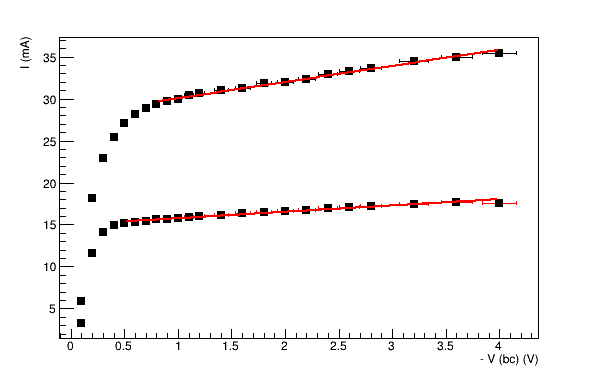
\includegraphics[width=0.4624\textwidth]{pictures/tot.png}
    \caption{\textit{\textcolor{gray}{Il grafico mostra le misure di tensione ottenute dal multimetro (in ascissa) e dall'oscilloscopio (in ordinata) per entrambe le caratteristiche, si evidenzia come la curva più in alto corrisponde ad una corrente sulla base di 200 $\mu\mathrm{A}$ mentre quella inferiore a 100 $\mu\mathrm{A}$.}}}
    \label{graph::i_tot}
\end{figure}


Nella tabella \ref{tab::risultati} si presentano valori dei parametri e i $\tilde\chi^2$ dei fit per la calibrazione e per le caratteristiche dei diodi.

\begin{table}[h!]
	\centering
  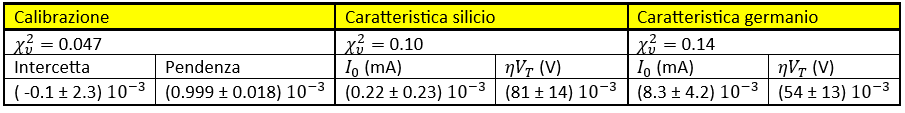
\includegraphics[width=1.\textwidth]{pictures/risultati2.png}	\caption{\textit{\textcolor{gray}{La tabella mostra i risultati ottenuti dai fit riportando da sinistra i risultati dalla calibrazione, la caratteristica del silicio e quella del germanio}}}
    \label{tab::risultati}
\end{table}


Nella seguente prova si è tentato di ricostruire le caratteristiche I-V di due diodi a semiconduttore (Si, Ge) in polarizzazione diretta. In aggiunta si è tentato di ricavare la corrente di saturazione inversa ed il prodotto fra il fattore di idealità e la tensione termica per le due componenti ottenendo [valori] con un accordo di [valori]. Inoltre è stata preventivamente compiuta anche una calibrazione degli strumenti di misurazione utilizzati per assicurarsi che non vi fosse uno sfasamento fittizio fra i due durante la fase di misurazione di una stessa grandezza ottenendo [valori] con un accordo di [valori].

\section*{Introduzione}
In questo esperimento è stata analizzata la caratteristica I-V di due diodi a semiconduttore, in silicio (Si) e germanio (Ge), variando l’intensità di corrente continua tramite un potenziometro. Un diodo a giunzione p-n consiste in due regioni contigue con drogaggi specifici, ottenuti introducendo impurezze in concentrazioni tipiche di $10^{14} - 10^{16} \, \mathrm{\frac{atomi}{cm^3}}$. 

La regione di tipo $n$ è drogata con atomi pentavalenti (come fosforo o arsenico), che forniscono elettroni aggiuntivi e aumentano la concentrazione di portatori di carica negativa. La regione di tipo $p$, invece, è drogata con atomi trivalenti (come boro o gallio), che creano lacune, ovvero assenza di elettroni, e agiscono come portatori di carica positiva.

Queste regioni, poste in contatto, generano una giunzione con un potenziale di contatto. Quando si applica una tensione esterna in polarizzazione diretta, questa riduce ulteriormente la barriera di potenziale, permettendo alle cariche libere (elettroni e lacune) di attraversare la giunzione facendo passare corrente. La caratteristica I-V di un diodo polarizzato direttamente segue un andamento esponenziale, descritto nel modello ideale dalla relazione\eqref{eq::diodo_ideale}:
\begin{equation}
\label{eq::diodo_ideale}
I=I_O(e^{\frac{V_D}{\eta V_T}}-1) \approx  I_O e^{\frac{V_D}{\eta V_T}}
\end{equation}

dove $I_0$ è la corrente di saturazione inversa, $V$ la tensione applicata, $V_T = \frac{kT}{q}$ la tensione termica, e $\eta$ il parametro di idealità del diodo, come discusso in [1].
 %controlla questa cosa, non mi piaceva nemmeno quando lo spiegava lei secondo me potrebbe influenzare in un qualche modo quanso abbiamo tensioni abbastanza piccole

Nella pratica, tuttavia, effetti di non idealità, come la resistenza del materiale semiconduttore e le perdite interne, alterano l’andamento della corrente ai valori più alti producendo correnti inferiori a quelle previste dal modello ideale.
	
\section{Medoto Sperimentale}
\section{Risultati}
\subsection{Dati}
\subsection{Analisi Dati}
Si è inoltre trascurato la costante unitaria presente all'interno della parentesi poichè il fattore esponenziale presente nella differenza risulta essere decisamente più grande.
\section{Conclusioni}
\section{Appendice}
\section{Bibliografia}
\end{document}
